

%Peter W.
%Requires the memoir class (as of this date v1.6180339e 2009/02/17)
%I suggest
\documentclass[oneside,11pt]{memoir}
%%% with the wide textblock, 12pt is too small for reading ease, so best not
%%% to use 11pt or 10pt.

%%% Arial
%\usepackage[T1]{fontenc}
%\usepackage[scaled]{uarial}
%\renewcommand*\familydefault{\sfdefault} %% Only if the base font of the document is to be sans serif

%%% Garamond
%\usepackage[T1]{fontenc}
%\usepackage{lmodern}
%\usepackage{garamond}

%%% MS San Serif
%\usepackage[T1]{fontenc}
%\usepackage[scaled]{helvet}
%\renewcommand*\familydefault{\sfdefault} %% Only if the base font of the document is to be sans serif

%%% Times
\usepackage{mathptmx}  % Times New Roman, but if you have Garamond then use it;
                       % you are writing a book, not a newspaper column
\DoubleSpacing         % memoir's double spacing
\usepackage{pwasu}     % this package

%%%%%%Added by Craig Picone to meet ASU's margin requirements
\usepackage{graphicx}    % needed for including graphics e.g. EPS, PS
\topmargin -0.2in        % read Lamport p.163
\oddsidemargin 0.5in   % read Lamport p.163
\evensidemargin 0in  % same as oddsidemargin but for left-hand pages
\textwidth 5.5in
\textheight 8.83in
%\pagestyle{empty}       % Uncomment if don't want page numbers
\parskip 7.2pt           % sets spacing between paragraphs
%\renewcommand{\baselinestretch}{1.5} % Uncomment for 1.5 spacing between lines
\parindent 0pt          % sets leading space for paragraphs
 %%%%%%%%

%    The general sequence in your document, after you have set the data for
%the TITLE and APPROVAL pages, and any other specifics in the preamble is:
\DoubleSpacing
\begin{document}
\maxtocdepth{subparagraph} % put everything into the ToC
\pagestyle{plain}  % pagestyle for the prelims
\frontmatter
\thetitlepage
%%\approvalpage

%% Added by bbailey1
% Macro for List of Symbols
\def\listofsymbols{%%%%%%%%%%%%%%%%%%%%%%%
%Sample List of Symbols
%%%%%%%%%%%%%%%%%%%%%%%
\begin{tabbing}
% YOU NEED TO ADD THE FIRST ONE MANUALLY TO ADJUST THE TABBING AND SPACES
$n$~~~~~\=\parbox{5in}{Vector size\dotfill \pageref{symbol:nml}}\\
%ADD THE REST OF SYMBOLS WITH THE HELP OF MACRO
\addsymbol m: {Vector size}{symbol:nml}
\addsymbol l: {Vector size}{symbol:nml}
\addsymbol x: {State vector}{symbol:x}
\addsymbol u: {Control input}{symbol:x}
\addsymbol y: {Output vector}{symbol:x}
% .
% .
% .
\addsymbol \mathbf{A}: {State Matrix}{symbol:A}
\addsymbol \mathbf{B}: {Input Matrix}{symbol:B}
\addsymbol \mathbf{C}: {Output Matrix}{symbol:C}
% .
% .
% .
% ALWAYS KEEP THE FOLLOWING LINE
\end{tabbing} \clearpage}
\def\addsymbol #1: #2#3{$#1$ \> \parbox{5.45in}{#2 \dotfill \pageref{#3}}\\}
\def\newnot#1{\label{#1}}


%%%%%%%%%%%%%%%%%%%%%%%%%%%%%%%%%%%%%%%%%%%%%%%%%%%%%%%%%%%%%%%%%%%
% here is the main part of your dessertation

% put your abstract here

\asuabstract
\setlength{\parindent}{.5in}
This is a sample abstract

% your acknowledgement

\setdedication{ Your dedication goes here. } % if you want a dedication

\asudedication

\asuacknowledgements
[Enter your text here]

\tableofcontents
\listoftables   % if you have any tables

\listoffigures  % if you have any figures

%% Added by bbailey1
%% Uncomment the next 3 lines for List of Symbols
% \newpage
% \chapter*{List of Symbols\hfill} \addcontentsline{toc}{chapter}{LIST OF SYMBOLS}
% \listofsymbols

%%
% Mark your variables in your source code with \newnot{YOUR_SYMBOL_LABEL}.
% Example:
% ...Here, if the dimensions of A \newnot{sybmol:A}, B \newnot{symbol:B}, and C \newnot{symbol:C} are
% nxn, nxm and lxn \newnot{symbol:nml} respectfully; then ...
%%

%\newpage
%\chapter*{PREFACE\hfill} \addcontentsline{toc}{chapter}{PREFACE}
%[Enter your text here]
%\clearpage

%% if you have more prelim sections, then
%%%\clearpage
%%%%%\pagestyle{plain}
%%%%%\prelimtitle   text % for sections after the ToC, etc, before main text
\mainmatter
\pagestyle{asu}

\addcontentsline{toc}{chapter}{CHAPTER}

\pagestyle{plain}
% finally, start of your main text

\chapter{INTRODUCTION}

\DoubleSpacing
\setlength{\parindent}{.5in}
Human interpersonal interactions are socially driven exchanges of verbal and non-verbal communicative cues. The essence of humans as social animals is very well exemplified in the way humans interact face-to-face with one another. Even in a brief exchange of eye gaze, humans communicate a lot of information about themselves, while assessing a lot about others around them. Though not much is spoken, plenty is always said. We still do not understand the nature of human communication and why face-to-face interactions are so significant for us.

Social interaction refers to any form of mutual communication between two individuals or between an individual and a group \cite{riggio_assessment_1986}. Such communications involve any or all forms of sensory and motor activities as deemed necessary by the participants of the interaction. Social, Behavioral and Developmental Sociologists emphasize that the ability of individuals to effectively control expressive behavior is essential for the social and interpersonal functioning of our society. Such social interactions are the aggregate cause of social behaviors, social actions and social contact that helps not only in effective bilateral communication, but also in forming an efficient feedback driven behavioral learning loop. It is this feedback (termed as social feedback) that children use towards developing good social and communicative skills.

Recent studies in behavioral psychology are furthering our understanding of the importance of social behaviors and social actions in everyday context. Researchers have revealed an unconscious need in humans to mimic and imitate the mannerisms of their interaction partners. An increasing number of experiments have highlighted this need for imitation to be very primeval and that they offer an elegant channel for building trust and confidence between individuals.

\section{Components of Social Interactions}
From a neurological perspective, social interactions result from the complex interplay of cognition, action and perception tasks within the human brain. For example, the simple act of shaking hands involves interactions of sensory, motor and cognitive events. Two individuals who engage in the act of shaking hands have to first make eye contact, exchange emotional desire to interact (this usually happens through a complex set of face and body gestures, such as smile and increased upper body movements), determine the exact distance between themselves, move appropriately towards each other maintaining Proxemics (interpersonal distance) that are befitting of their cultural setting, engage in shaking hands, and finally, move apart assuming a conversational distance which is invariably wider than the hand shake distance. Verbal exchanges may occur before, during or after the hand shake itself. This example shows the need for sensory (visual senses of face and bodily actions, auditory verbal exchange etc.), perceptual (understanding expressions, distance between individuals etc.), and cognitive (recognizing the desire to interact, engaging in verbal communication etc.) exchange during social interactions. Further, though social interactions display such complex interplay, they have been studied in the human communication literature under two important categories \cite{brent_d._ruben_human_1975}, namely,

\begin{itemize}
\item \emph {Verbal communication}: Explicit communication through the use of words in the form of speech or transcript.
\item \emph {Non-verbal communication}: Implicit communication cues that use prosody, body kinesis, facial movements and spatial location to communicate information that may be unique or overlapping with verbal information.
\end{itemize}

While the spoken language plays an important role in communication, speech accounts for only 35\% of the interpersonal exchanges. Nearly 65\% of all information communication happens through non-verbal cues \cite{knapp_nonverbal_1996}. Out of this large chunk, 48\% of the communication, is through visual encoding of face and body kinesis and posture, while the rest is encoded in the prosody (intonation, pitch, pace and loudness of voice) \cite{borkenau_thin_2004}. A closer look at the various non-verbal communication modes can highlight the importance of the multi-modality of social exchanges (See Figure \ref{Fig:Figure1}).

\subsection{Non-verbal communication cues}
Speech, voice, face and body form the primary channels of communication in any social interaction. Speech forms the primary channel for verbal communication, while prosody (intonation, pace and loudness of one's voice), face, and body (posture, gesture and mannerisms) form the medium for nonverbal communication. In everyday social interactions, people communicate so effortlessly through both verbal and non-verbal cues that they are not cognizant of the complex interplay of their voice, face and body in establishing a smooth communication channel.

\begin{figure}[h]
\begin{center}
 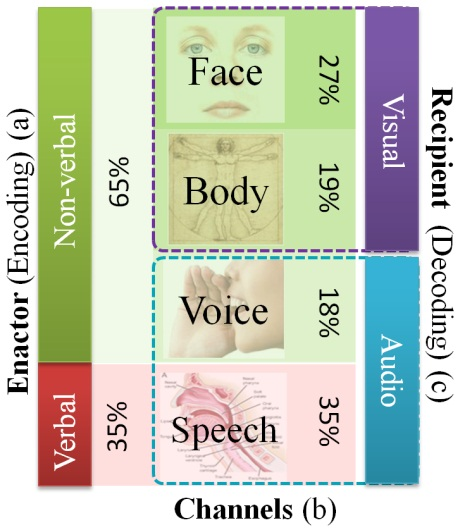
\includegraphics[width=3in]{NVCEncodings.jpg}
\end{center}
\caption{Relative importance of a) verbal vs. non-verbal cues, b) four channels of non-verbal cues, and c) visual vs. audio encoding and decoding of bilateral human interpersonal communicative cues.}
\label{Fig:Figure1}
\end{figure}

\subsubsection{Social Sight and Social Hearing}
Unlike speech, which is mostly under the conscious control of the user, the non-verbal communication channels are engaged from a subconscious level. Though people can increase their control on these channels through training, innately, individuals demonstrate certain inability to control their non-verbal cues. This inability to control non-verbal channels is referred to as the leakiness \cite{brown_social_1986} and humans (evolutionarily) have learnt to pick up these leaked signals during social interactions. For example, people can read very subtle body mannerisms very easily to determine the mental state of their interaction partner. Eye Gaze is a classic example of such subtle cues where interaction partners can detect interest, focus, involvement and role play, to name a few.  On this leakiness scale, it has been found that the voice is the leakiest of all channels, implying that emotions of individuals are revealed first in their voice before any of the other channels are engaged. The voice is followed by body, face and finally the verbal channel, speech. The leakiness is plotted on the abscissa of Figure \ref{Fig:Figure2} with the ordinate showing the amount of information encoded in the other three non-verbal communication channels. It can be seen that the face communicates the most amount of non-verbal cues, while the prosody (voice) is the first channel to leak emotional information.

\begin{figure}[h]
\begin{center}
 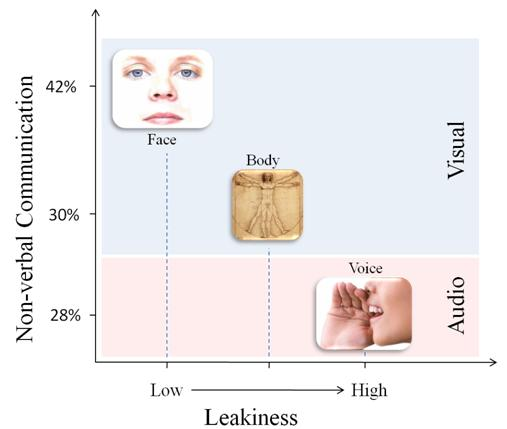
\includegraphics[width=4in]{Leakiness.jpg}
\caption{Relative communicative information plotted against its leakiness. Speech forms the verbal channel. Face, body and voice form the non-verbal communication channels.}
\label{Fig:Figure2}
\end{center}
\end{figure}

\subsubsection{Social Touch}
Apart from visual and auditory channels of social stimulation, humans increasingly rely on social touch during interpersonal interactions. For example, hand shake represents an important aspect of social communication conveying confidence, trust, dominance and other important personal and professional skills \cite{burgoon_relational_1984}. Social touch has also been studied by psychologists in the context of emotional gratification. Wetzel \cite{wetzel_midas_1984} demonstrated patron gratification effects through tipping behavior when waitresses touched their patrons. Similar studies have revealed the importance of social touch and how conscious decision making is connected deeply with the human affect system. In the recent years social touch has gained a lot of interest in the area enriching remote interactions \cite{haans_mediated_2006} \cite{bailenson_virtual_2008} to help better understand an individual's  social awareness and social presence. In the next section, we describe the term \emph{Social Situational Awareness} as seen pertinent to this report and emphasize the importance of any individual being aware of his/her social situational awareness.

\section{Social Situational Awareness}
We refer to the term Social Situational Awareness (SSA) as the ability of individuals to receive the visual, auditory and touch based non-verbal cues and respond appropriately through their voice, face and/or body (touch and gestures). Figure \ref{Fig:Figure3} represents the concept of consuming social cues and reacting accordingly to the needs of social interaction. Social cognition bridges stimulation and reciprocation and allows individuals to interpret and react to the non-verbal cues.

\begin{figure}[h]
\begin{center}
 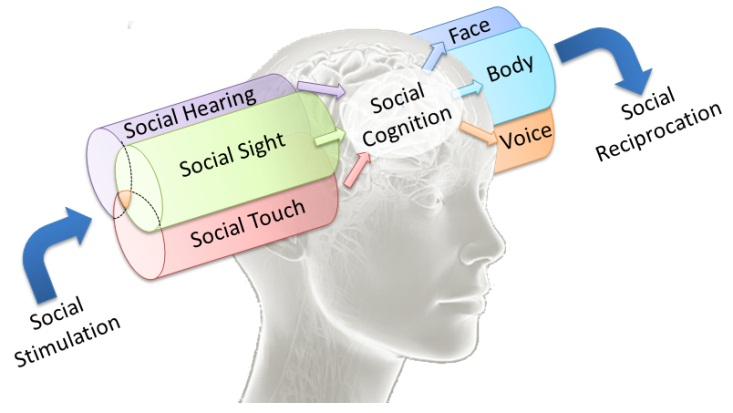
\includegraphics[width=4.5in]{SSA.jpg}
 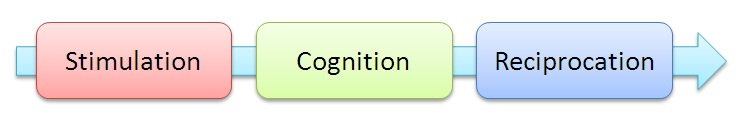
\includegraphics[width=4.5in]{SSA2.jpg}
\caption{Social Situational Awareness.}
\label{Fig:Figure3}
\end{center}
\end{figure}

The Transactional Communication Model \cite{sameroff_reproductive_1975} suggests that during any face-to-face interaction, the interpretation of the social stimulation and the corresponding social response are under the control of various factors including the culture, physical and emotional state, experience, memory, expectation, self concept and attitude of the individuals involved in the interaction. In order to effectively cognize and react to the social stimulation, it is necessary that individuals be able to receive and synthesize these above factors. Enriching social situational awareness then represents the ability of a mediator (telecommunication technology for remote interactions; social assistive technologies for the disabled population) to allow the social cognition of an individual to have access to the above mentioned factors and thereby evoking appropriate social reciprocation.

\subsection{Social Situational Awareness in Everyday Social Interactions}
\subsubsection{SSA in Dyadic Interactions}
Human communication theories have studied dyadic or bilateral interaction between individuals as the basis of most communication models. Theories of leadership, conflict and trust base their findings on dyadic interaction primitives where the importance of the various non-verbal cues is heightened due to the one-on-one nature of dyadic interactions. Eye contact, head gestures (nod and shake), body posture (conveying dominance or submissiveness), social touch (hand shake, shoulder pat, hug, etc.), facial expressions and mannerisms (smile, surprise, inquiry, etc.), eye gestures (threatened gaze, inquisitive gaze, etc.) are some of the parameters that are studied closely in dyadic understanding of human bilateral communication \cite{altmann_analysis_2007}. Enriching SSA in dyadic communication thus focuses on appropriate extraction and delivery of communicator's face, body and voice based behaviors to a remote participant or to a person who is disabled.

\subsubsection{SSA in Group Interactions}
Group dynamics refer to the interactions between members of a team assembled together for a common purpose. For example, teams of medical professionals operating on a patient, a professional team meeting for achieving a certain goal, a congressional meeting on regulations, etc. represent groups of individuals with a shared mental model of what needs to be accomplished. Within such groups, communication behaviors play a vital role in determining the dynamics and outcome of the meeting. Zancanaro et. al. \cite{zancanaro_automatic_2006} and Dong et. al.  \cite{dong_using_2007} presented one model of identifying role-play of participants in a group discussion. They identified two distinct categories of roles for the individuals within the group, namely, the socio-emotion roles and the task roles. The socio-emotional roles included the protagonist, attacker, supporter and neutral, and the task roles included the orienteer, seeker, follower and giver. These roles were dependent heavily on the emotional state (affect) of the individuals participating in the group interaction. Good teams are those where individual team members and their leaders are able to compose and coordinate their affect towards a smooth and conflict free group interaction. And effective leaders are those who can read the affect of their group member, make decisions on individual's roles and steer the group towards effective and successful decisions. Inability to access the affective cues of team members has significant consequences to team leaders leading to unresolved conflict situations and underproductive meetings, or in the worst case, the death of a patient. Thus, enriching SSA in group settings correspond to the extraction and delivery of team's interaction dynamics (which are in turn modulated in their mutual and group affect) to a remotely located team member or to a co-located individual who is disabled.

In essence, SSA enrichment technologies provide for a richer interaction experience for individuals involved either in a dyadic or group interaction. It is well established that in teams comprising of good communication strategies a shared mental model towards effective decision is achieved faster with little or no emotional stress on the team members. The lack of social awareness can lead to interactions where individuals are not committed cognitively and find it very difficult to focus their attention on the communication. This is true in the case of remote interactions, disability and situations where doctors, nurses and other medical professionals are operating simultaneously on a patient.

\subsection{Learning Social Awareness}
Figure \ref{Fig:Figure3} represents a simple unidirectional model of social stimulation and reciprocation. In reality, social awareness is a continuous feedback learning system where individuals are learning through observing, predicting, enacting and correcting themselves. It is this learning mechanism that allows people to adapt easily from one culture to another with ease - here we refer to term culture in very broadly encompassing work culture, social culture in a new environment and culture of a new team, etc. Figure \ref{Fig:Figure4} shows the continuous feedback loop involved in social learning systems, based on the model of human cognition as proposed by Hawkins \cite{hawkins_intelligence_2004}.

\begin{figure}[h]
\begin{center}
 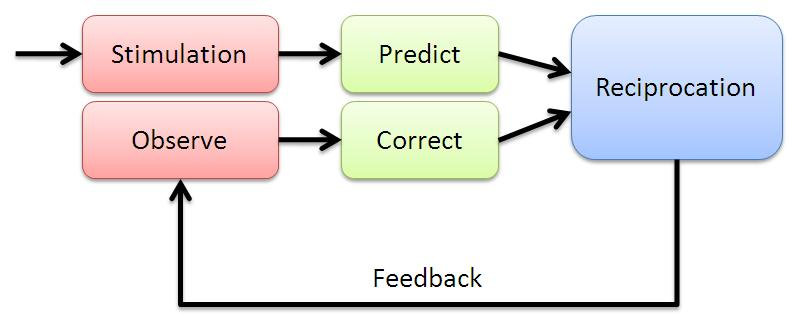
\includegraphics[width=4.5in]{SSALearning.jpg} 
\caption{Social learning systems with continuous learning feedback loop.}
\label{Fig:Figure4}
\end{center}
\end{figure}

People exposed to everyday social interactions learn social skills from the three different social stimulations (social sight, social hearing and social touch) effortlessly. When faced with a new environment, individuals exercise their learned social skills to predict what social actions are appropriate in the setting. Once executed, they observe and assess their counterparts to determine if their new behavior is appropriate or not for the new setting. Such learning continues until their social rule set adapts to the new environment. Psychologists have been studying the nature of learning that happens in individuals who move from Western to Eastern cultures and vice versa. Largely, USA and Japan have been the countries of choice based on their economic equality and cultural diversity \cite{rogers_edward_2002}. In the West, large body movements and excitement in the voice are considered to be typical and to a large part encouraged as a good social skill. Similar attitudes in the East are considered to be inappropriate in professional settings and to a large extent considered indecent. An individual displaying any such inappropriate mannerisms or gestures will receive social feedback from his counterparts (everyone staring at the individual, reduced interaction with the individual, etc.).  Thus, social awareness is a learned set of rules about the environment within which the individual is present and this requires continuous monitoring of the various social channels of stimulation. Deprivation of any one of these channels can in turn affect the ability of the individual to learn social actions and responses that are pertinent to a social situation. Thus, enriching SSA not only offers the means for individuals to make appropriate social decisions, but also cognitively trains them towards effective social judgments.

-------------------------------------
In this paper, we advocate that the social separation induced by remote interactions in physically separated partners is similar to the social separation resulting from information impoverishment induced by sensory/physical disabilities in co-located interaction partners and propose technologies targeted at enriching social interactions.
--------------------------------------




\chapter{RELATED WORK}

\DoubleSpacing
\setlength{\parindent}{.5in}
[Enter your text here]

\section{Test 1}
\subsection{Test 2}
\subsubsection{Test 3}

\clearpage


%\newpage
\vspace*{1in}
%\chapter*{REFERENCES\hfill} \addcontentsline{toc}{chapter}{REFERENCES}
\begin{SingleSpace}
\bibliographystyle{ieeetr}	
\bibliography{references}
\end{SingleSpace}
%\clearpage

%% maybe endnotes
%% maybe bibliography
% if appendices, then

\appendix
\addcontentsline{toc}{chapter}{APPENDIX}
\chapter{\uppercase{Insert Appendix A Title here}}
\clearpage
\chapter{\uppercase{Insert Appendix B Title here}}
\clearpage

% if Biographical sketch then
%\newpage
%\newpage
%\begin{center}\bibname\end{center} \addcontentsline{toc}{chapter}{\bibname}
%\clearpage
%[Enter your text here]
%\clearpage
%\newpage	

This LaTeX document was generated using the Graduate College Format Advising tool. Please turn a copy of this page in when you submit your document to Graduate College format advising. You may discard this page once you have printed your final document. DO NOT TURN THIS PAGE IN WITH YOUR FINAL DOCUMENT!


\end{document}		
		